\documentclass[10pt,letterpaper]{article}
\usepackage[spanish]{babel}
\usepackage[utf8x]{inputenc}
\usepackage{fancyvrb}
\usepackage{fancyhdr}
\usepackage{url}
\usepackage{verbatim}
\usepackage{graphicx}
\usepackage{rotating}
\usepackage{listings}


\lstset{
language=C
}

\parskip 1mm
\setlength{\topmargin}{0pt}
\oddsidemargin  0.5cm
\evensidemargin 0.5cm
\textwidth      15.5cm
\textheight     21.0cm
\headsep        4 mm
\parindent      0.5cm

\pagestyle{fancyplain}

\lhead{Taller de Herramientas de Modelado de Procesos de Negocio}
\rhead{\bf \it Proyecto N$°$2, Etapa 0 }
\lfoot{}
\cfoot{}
\rfoot{\bf \thepage}
\renewcommand{\footrulewidth}{0.4pt}

\title{Taller de Herramientas de Modelado de Procesos de Negocio \\ Proyecto N$°$2, Etapa 0}
\author{Patricia Fredes (2584080-1) \\ María Jose Fuentes (2873042-k) \\ Margarita Ortega (2773024-8) \\ Fernando Morales (2573034-8)}

\date{\vspace*{1cm} Valparaí­so, Septiembre del 2012}

\newpage

\begin{document}
\maketitle
\thispagestyle{empty}
\newpage
\tableofcontents

\makeatother

\newpage

\section{Introducción}
En este informe se realiza el modelado de los procesos de negocio de la panadería Rodenas que está ubicada en Rancagua, donde fabrica, vende y distribuye sus productos a lo largo de gran parte de la provincia del Cachapoal. Nace 1948 aproximadamente, en la localidad de Coya desde donde se expande hacia la ciudad de Rancagua, por la iniciativa e involucramiento de los hijos del fundador. En este momento va en la tercera generación de gestión, teniendo 20 trabajadores repartidos en distintos turnos, y otras panaderias con el mismo nombre pero sin relacion comercial con la panaderia en estudio, los lazos son meramente familiares.
Como misión manifiesta la de producir y vender pan de buena sabor, aspecto y duradero en el tiempo. Entregando productos de calidad en la región manteniendo la costumbre chilena en la fabricación de este.
La filosofía de la empresa con respecto a sus proyecciones o visión es bastante limitada. Manteniendo la postura de “vivir el día a día”, acortando la mirada a plazos lo más pequeño posible posible. De esta manera se ha mantenido más de 60 años funcionando, con todos los altos y bajos que ha manifestado la industria.
\\
Para efectos de este proyecto, se ha incorporado la sección ``reposteria", la cual se encarga de producir tortas, pasteles y galletas. Cabe destacar que son procesos extraidos de la panadería del supermercado Hiper Lider 15 norte de la ciudad de Viña del mar. Si bien, la diferencia en cuanto a tamaño de ambos, es grande, el proceso que se debe hacer para su producción es el mismo. \\
Además es posible que este mecanismo tambien ayude a la empresa de panadería ampliar sus rangos de venta hacia la repostería.

\section{Herramienta}
La herramienta que se utilizará para realizar el modelo de los procesos de negocios de la panadería Rodenas es el software \textbf{"Bizagi Process Modeler"}.

%\newpage
\section{Procesos de nivel 1}
\subsection{Actores y roles}
\begin{itemize}
\item \textbf{Administrador:} Es la cabeza de la empresa y el punto de control en el maximo de procesos que puede involucrarse, por esto la desiciones de la empresa pasan todas por él. Tambien se preocupa del abastecimiento de insumos y de la mantencion de los recursos. 

\item \textbf{Vendedoras:} En la sala de venta se preocupan de ser el primer contacto con los clientes, dandole accesos a los productos y cuantificandolos en dinero para que el cliente pueda pagar.

\item \textbf{Cajero:} La unica tarea de esta persona es cobrar el dinero en la sala  de venta. Siendo  la persona de confianza en la sala de venta del administrador, pero sin tener poder de desición en este lugar.

\item \textbf{Repartidores:} Se encargan de ser el nexo entre la panadería y la distribución de pan a mayor escala. Distribuyen el pan, cobran en algunos casos y tienen la potestad de poder hacer nuevos clientes de gran escala.
\end{itemize}

\subsection{Modelos de procesos a nivel de Macro procesos}
La panadería Rodenas se dedica a la fabricación, venta y distribución de pan y reposteria. A nivel macro todo empieza con una solicitud diaria que da el inicio al trabajo, pasando por el proceso de fabricación de pan (Producción de pan) y el proceso de fabricación de reposteria (Producción de reposteria), una vez terminados estos procesos pueden pasar a la Distribución o Ventas dependiendo de que prioridad tiene cada uno en el mismo momento, esto pasa por una decisión del Administrador. Después tenemos el proceso Ventas que se encarga de la venta del pan, venta de resposteria y atención al cliente, pero puede suceder que el proceso de Ventas antes que termine se vea entorpecido por si falta o no pan o reposteria, aquí es donde vuelve al proceso de Producción y se realiza nuevamente el flujo. Paralelo a este proceso tenemos Distribución, que es el encargado de tomar los pedidos durante el día y terminar el flujo diario.

\begin{center}
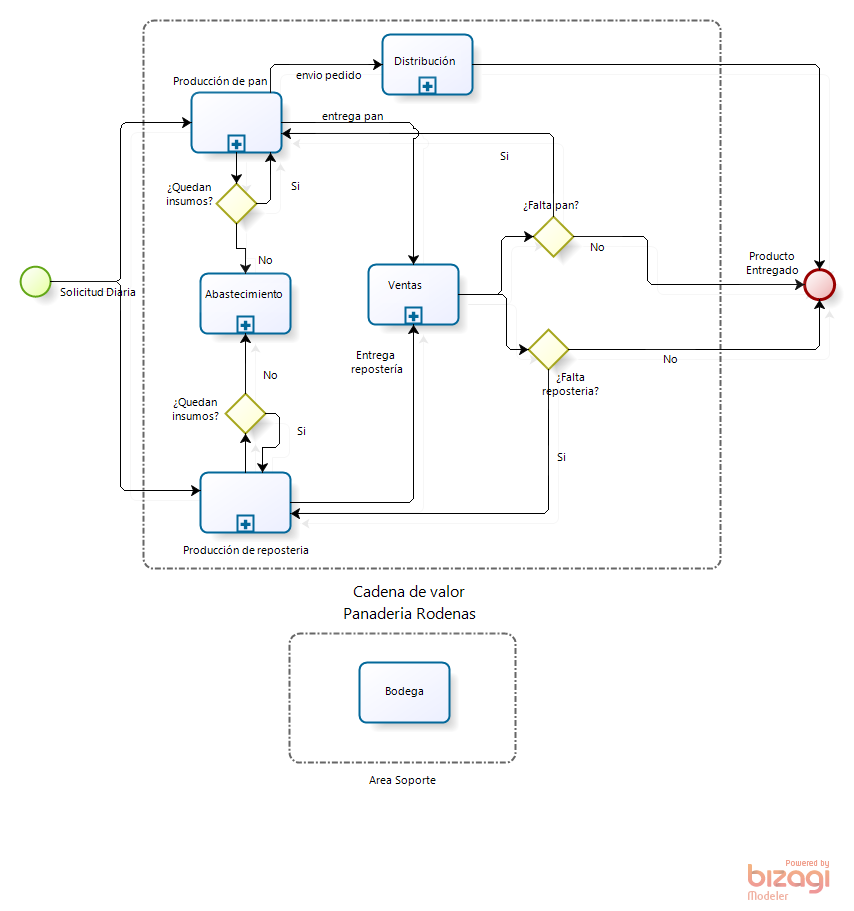
\includegraphics[width=15cm]{./imagenes/Macro_proceso.png}\\
Figura 1: Macro-proceso de panadería Rodenas.
\end{center}
\subsection{Descripción de modelos de procesos nivel 1} 


\section{Indicadores}
\begin{itemize}

\item \textbf{Cantidad de solicitud de pan para la distribución:}
\\
\\
Con este indicador se tiene la posibilidad de ver que tan importante es la recepci\'on de solicitud de pedidos por parte del cliente hacia el repartidor espec\'ifico, en caso de que sean muchos, es decir, la panadería se expanda hacia otros sectores de Rancagua o de la región, se puede analizar la posibilidad de modificar el proceso de recepci\'on de pedido e intentar que mediante tecnologías de la información modificar alg\'un  proceso con tal de hacer mas \'agil, r\'apido y eficiente la toma de pedidos. De acuerdo a esto, se puede medir, luego de optimizar, si la cantidad de solicitudes aumentan usando este tipo de herramientas.
\\
\item \textbf{Cantidad de pan vendido v/s pan que sale de producción hacia la sala de ventas:}
\\
\\
En este aspecto, se puede verificar si exite la necesidad de incrementar o disminuir la producci\'on de pan, ya sea para la sala de ventas o para la distribución a clientes, de acuerdo al dia y fecha en cuanto a demanda de pan. De acuerdo a esto, se puede comprobar las perdidas asociadas a la producción innecesaria y a raiz de esto mejorar el proceso de abastecimiento, a fin de eliminar costos in\'utiles.
\\
\item \textbf{Calidad del pan:}
\\
\\
La calidad del pan, medible de acuerdo a la satisfacción del cliente, sin duda es un aspecto importante para mantener a flote el negocio. Es por esto, que el proceso de producción de pan, debe ser ciudadosamente observado, a fin de mantener los estandares de calidad que la politica de la empresa posee. Para optimizar este seguimiento, se pueden utilizar varias herramientas que pueden ser incorporadas en un nuevo proceso pequeño de control de calidad. 
\\
\item \textbf{Tiempo de ejecución de las tareas:}
\\
\\
El tiempo de ejecución va directamente asociado al indicador de calidad del producto, en ese aspecto, vinculado al proceso de control de calidad, se podrían realizar procesos paralelos y en conjunto de tecnologías de la información agilizar el proceso de la panadería.

\end{itemize}


\section{Conclusiones}
En cuanto a las conclusiones podemos decir, que modelar los procesos de una panadería es especialmente ideal, puesto que posee claramente identificados los roles de cada participante de las actividades que se deben realizar.\\
Se observa que la mayor parte de los procesos tienen como responsable al administrador de la organización, por lo que como mejora, si es que la carga es muy grande, se podría delegar esta responsabilidad a otra persona siendo el administrador solo supervisor de los procesos.\\
Por otro lado, como lo describimos al comienzo, si se realizan los cambios y extensiones pertinentes, es posible ampliar el rango de ventas de la panaderia, añadiendo una sección repostería que permitiera vender tortas, galletas y/o pasteles.\\
En cuanto a la herramienta utilizada, es bastante fácil de utilizar, pues contiene todos los elementos de la notación BPMN 2.0 y está especialmente diseñado para este fin, en contraste con la herramienta ProcessMaker, la cual es un poco menos intuitiva además de no incorporar todos los elementos necesarios para el modelamiento, pero si para gestionarlos.

\bibliographystyle{alpha}
\bibliography{bibbase}
 
\end{document}
